
	\appendix
	\chapter{Basic facts in topological dynamics}
	\chaptermark{Topological dynamics}
	\label{app:topdyn}
	In this section, we build the framework for topological dynamics in the generality needed in the thesis. The majority of the facts proven here are folklore, and their proofs are, for the most part, straightforward adaptations of the proofs from \cite{Gl76}, where the main focus is on flows of the form $(G,\beta G)$. Since I have not found them in the literature in the required generality, they are included in the thesis, with complete proofs, for the convenience of the reader (and possibly future reference).
	
	The definitions also essentially the same as in \cite{Gl76}; the only nontrivial change is the definition of the operation $\circ$ --- see Definition~\ref{dfn:circ} --- as the one introduced in \cite[Section IX.1]{Gl76} does not seem generalise to arbitrary Ellis groups (but the two definitions coincide in the case of $(G,\beta G)$, see Remark~\ref{rem:circ_equivalence}).
	\subsection*{Preparatory facts}
	
	
	\begin{dfn}
		\index{ideal}
		\index{left ideal}
		A (left) ideal $I\unlhd S$ in a semigroup $S$ is a subset such that $IS\subseteq I$.\xqed{\lozenge}
	\end{dfn}
	
	
	\begin{dfn}
		\index{semitopological group}
		A group $G$ endowed with a topology is a \emph{semitopological group} if multiplication is separately continuous in $G$.
		\xqed{\lozenge}
	\end{dfn}
	
	\begin{rem}
		\label{rem:semitop_acts_on_itself}
		Note that, as an immediate consequence of the definition, semitopological group acts on itself by homeomorphisms by left and right multiplication, as well as by conjugation. In particular, inner automorphisms are homeomorphisms.\xqed{\lozenge}
	\end{rem}
	
	\begin{dfn}
		\index{left topological semigroup}
		A semigroup $S$ equipped with a topology is called a \emph{left topological semigroup} if the multiplication is continuous on the left, i.e.\ for every $s_0\in S$, the map $s\mapsto ss_0$ is continuous.
		\xqed{\lozenge}
	\end{dfn}
	
	\begin{ex}
		For every topological space $X$, the semigroup of functions $X^X$ with pointwise convergence (i.e.\ Tychonoff product) topology is a left topological semigroup.
		\xqed{\lozenge}
	\end{ex}
	
	\begin{fct}[Ellis joint continuity theorem]
		\label{fct:ellis_joint_cont}
		Suppose $G$ is a locally compact Hausdorff semitopological group. Then $G$ is a topological group (i.e.\ multiplication is jointly continuous and inversion is continuous).
	\end{fct}
	\begin{proof}
		This is \cite[Theorem 2]{ellis57}.
	\end{proof}
	
	\begin{fct}
		\label{fct:elementary_algebra}
		If $S$ is a semigroup and $S$ has a left identity element and left inverses, then $S$ is a group.
	\end{fct}
	\begin{proof}
		Let $e$ be a left identity in $S$, and let $a\in S$ be arbitrary. If $b$ is the left inverse of $a$, it is enough to show that $ae=a$ and $ab=e$.
		
		Let $c$ be the left inverse of $b$, so that $ba=cb=e$.
		
		Then
		\[
			e=cb=c(eb)=c(ba)b=(cb)(ab)=e(ab)=ab,
		\]
		and thus
		\[
			ae=a(ba)=(ab)a=ea=a.\qedhere
		\]
	\end{proof}
	
	\begin{fct}
		\label{fct:minimal_ideals_idempotents}
		Suppose $S$ is a semigroup with a compact $T_1$ topology such that for any $s_0\in S$, the map $s\mapsto ss_0$ is continuous and a closed mapping (the latter follows immediately from continuity and compactness if $S$ is Hausdorff).
		
		Then there is a minimal (left) ideal $\cM$ in $S$ (i.e.\ a minimal set such that $S\cM=\cM$), and every such $\cM$ satisfies the following:
		\begin{enumerate}
			\item
			every $s\in \cM$ generates it as a left ideal: $\cM=Ss$ (thus, by the assumptions, $\cM$ is closed),
			\item
			\index{idempotent}
			if $u\in \cM$ is an idempotent (i.e.\ it satisfies $uu=u$), then $u\cM$ is a group (with composition as group operation and $u$ as identity),
			\item
			each $\cM$ is the disjoint union $\bigsqcup_{u} u\cM$, where $u$ ranges over idempotents $u\in \cM$; in particular, idempotents exist,
			\item
			for every idempotent $u\in \cM$ and every $s\in \cM$, we have that $su=s$,
			\item
			given two idempotents $u,v\in \cM$, the map $s\mapsto vs$ defines an isomorphism $u\cM\to v\cM$
			\item
			every two groups of the form $v\cN$ (where $\cN$ is a minimal left ideal in $S$ and $v$ is an idempotent in $\cN$) in $S$ are isomorphic as groups (even if they are contained in distinct ideals).
		\end{enumerate}
	\end{fct}
	\begin{proof}
		(The proof below is the same as in the case of compact Hausdorff left topological semigroups, which is classical.)
		
		Note that if $S'\subseteq S$ is a closed subsemigroup, then $S'$ also satisfies the hypotheses of the fact we are proving.
		
		For existence of minimal left ideals, notice that by the assumption, principal left ideals in $S$ (i.e.\ ideals of the form $Ss_0$ for some $s_0\in S$) are compact, so it is not hard to see that the family of all principal left ideals satisfies the assumptions of the Kuratowski-Zorn Lemma. This implies the existence of minimal principal left ideals. But every ideal contains a principal ideal, so the minimal principal left ideals are also minimal left ideals.
		
		Now, fix a minimal (left) ideal $\cM\unlhd S$.
		
		(1) follows easily from the minimality assumption: if $a\in \cM$, then $Sa\subseteq \cM$ is an ideal.
		
		(2): Clearly, $u\cM$ is a semigroup, and $u$ is a left identity. By Fact~\ref{fct:elementary_algebra}, it is enough to show that $u\cM$ has left inverses. But if $f\in u\cM$ is arbitrary, then by minimality of $\cM$, we have $\cM f=\cM$, so $u\cM f=u\cM$, so $u\in u\cM f$, i.e.\ for some $g\in \cM$ we have $(ug)f=u$.
		
		(3): Applying the Kuratowski's Lemma again, there is a minimal closed subsemigrup $K\leq \cM$. Pick any $u\in K$. Then $Ku\subseteq K$ is closed, and trivially, $Ku$ is a semigroup, so by minimality, $Ku=K$, so there is some $k\in K$ such that $ku=u$. But the set of all such $k$ is closed (by left continuity of multiplication and the $T_1$ assumption) and a subsemigroup of $K$, so it is just $K$ itself. In particular, $uu=u$, so $u$ is an idempotent.
		
		It follows that if $u\cM\cap v\cM\neq \emptyset$, then $u=v$ (indeed, if $f\in u\cM\cap v\cM$, then by (2) we have $f'\in \cM$ such that $ff'=u$, and it follows that $u\in v\cM f'=v\cM$; since $v\cM$ is a group, the only idempotent in it is $v$, so $u=v$).
		
		Finally, take any $m\in \cM$. We need to show that $m\in u\cM$ for some idempotent $u$. But the set of $f\in \cM$ such that $fm=m$ is a nonempty (because $\cM m=\cM$), closed subsemigroup of $\cM$, so it satisfies the assumptions of the fact we are proving, and so, by (3), it must contain an idempotent $u$. But then $m=um\in u\cM$.
		
		(4): Fix $u,s$. Then by minimality, $\cM=\cM u$, so there is some $s'\in \cM$ such that $s'u=s$. But then $su=(s'u)u=s'(uu)=s'u=s$.
		
		(5): Fix any idempotents $u,v\in \cM$. Then $uv=u$ and $vu=v$, so $s\mapsto us$, $v\cM\to u\cM$ and $s\mapsto vs$, $u\cM\to v\cM$ are inverse to one another, so they are bijections. Furthermore, it is easy to see that they are homomorphisms, as by the preceding point, for any $f,g\in \cM$ we have $ufug=ufg$ and $vfvg=vfg$.
		
		(6): By (5), it is enough to show that for every $u\in \cM$ and every minimal left ideal $\mathcal N$, there is an idempotent $v\in \mathcal N$ such that $v\mathcal N\cong u\cM$. First, note that $\mathcal N u$ is a left ideal contained in $\cM=Su$, so $\mathcal N u=\cM$, and there is some $f\in \mathcal N$ such that $fu=u$. The set of all such $f$ is a closed subsemigroup of $\mathcal N$, so it contains an idempotent $v$ by (3). Thus, we have $vu=u$. By analogous consideration, there is an idempotent $u'\in \cM$ such that $u'v=v$. But then $u=vu=(u'v)u=u'(vu)=u'u=u'$ (by (4)), so in fact $uv=v$. Similarly to (5), we conclude that $s\mapsto su$ yields a homomorphism $v\mathcal N\to u\cM$ with inverse $s\mapsto sv$.
	\end{proof}
	\index{u@$u$}
	\index{M@$\cM$}
	Throughout, we denote minimal ideals by $\cM$ or $\cN$ and idempotents in minimal ideals by $u$ or $v$.
	
	\begin{rem}
		\label{rem:explicit_ellisgroup_isomorphism}
		It is easy to see from the proof of Fact~\ref{fct:minimal_ideals_idempotents}(6), for arbitrary ideal groups $u\cM,v\cN$, we have an isomorphism $u\cM\to v\mathcal N$ given by $s\mapsto vsv$.\xqed{\lozenge}
	\end{rem}
	
	\begin{dfn}
		\index{ideal group}
		If $S$ is a semigroup as above, $\cM$ is a minimal left ideal, while $u\in \cM$ is an idempotent, we call $u\cM$ an \emph{ideal group} of $S$. By ``the" ideal group of $S$ we mean the unique isomorphism type of an ideal group of $S$.
		\xqed{\lozenge}
	\end{dfn}
	
	
	\begin{fct}
		Suppose $G$ is a semitopological group. If $A\subseteq G$, then $\overline{A}=\bigcap_V V^{-1}A$, where $V$ ranges over the neighbourhoods of the identity in $G$.
	\end{fct}
	\begin{proof}
		Fix any $V\ni e$. Let $x\in \overline{A}$. Then $Vx$ is a neighbourhood of $x$, so $Vx\cap A\neq \emptyset$, and thus $x\in V^{-1}A$.
		
		On the other hand, if $x\in V^{-1}A$ for every neighbourhood $V$ of $e$, then also $Vx\cap A\neq\emptyset$, so $V\cap Ax^{-1}\neq\emptyset$. Since $V$ was an arbitrary neighbourhood of $e$, by Remark~\ref{rem:semitop_acts_on_itself}, it follows that $e\in \overline{Ax^{-1}}=\overline{A} x^{-1}$, so $ex=x\in \overline{A}$.
	\end{proof}
	
	\begin{fct}
		\label{fct:semitop_T2_quot}
		\index{H(G)@$H(G)$}
		Suppose $G$ is a compact $T_1$ semitopological group. Then the derived subgroup $H(G):=\bigcap_V \overline V$ (where the intersection runs over all neighbourhoods of the identity in $G$) is a closed normal subgroup of $G$
		
		Furthermore, $G/H(G)$ is a compact Hausdorff topological group.
	\end{fct}
	\begin{proof}
		The proof is essentially given in \cite{Gl76} for the special case of the Ellis groups of a certain class of dynamical systems. We present the full proof for completeness.
		
		Recall that a semitopological group acts on itself by homeomorphisms on the left and on the right (Remark~\ref{rem:semitop_acts_on_itself}). For brevity, write $H$ for $H(G)$. It is clear by definition that $H$ is closed and contains the identity $e\in G$.
		
		\begin{clm*}
			If $V$ is an open neighbourhood of the identity $e\in G$, then $\overline{V}H\subseteq \overline{V}$.
		\end{clm*}
		\begin{clmproof}
			Choose any $v\in \overline{V}$. Then for any open $W\ni e$, we have $Wv\cap V\neq \emptyset$ (because $v\in Wv\cap \overline{V}$ and $Wv$ is open), so $wv\in V$ for some $w\in W$. But then by continuity, there is some open $U\ni e$ such that $wvU\subseteq V$, so $wv\overline{U}=\overline{wvU}\subseteq\overline V$ But by definition of $H$, we have $H\subseteq \overline{U}$, so $wvH\subseteq \overline{V}$, so $vH\subseteq w^{-1}\overline{V}\subseteq W^{-1}\overline{V}$. But since $v$ and $W$ were arbitrary, by the preceding fact, $\overline{V}H\subseteq \overline{\overline{V}}=\overline{V}$.
		\end{clmproof}
		By taking the intersection over all $V$ in the claim, we have that $H^2=HH\subseteq H$, so $H$ is a subsemigroup of $G$. It follows that for every $h\in H$, $hH$ is also a subsemigroup. Because multiplication by $h$ is a homeomorphism, $hH$ is also closed (and thus compact). Furthermore, since multiplication by any element of $G$ is a homeomorphism, $hH$ satisfies the assumptions of Fact~\ref{fct:minimal_ideals_idempotents}, so it contains an idempotent. But the only idempotent in $G$ is the identity, so $hH$ contains the identity, and hence $H$ must contain the inverse of $h$. Since $h$ was arbitrary, $H$ is a group.
		
		The fact that $H$ is normal follows immediately from the fact that inner automorphisms are homeomorphisms (cf.\ Remark~\ref{rem:semitop_acts_on_itself}) and they fix the identity.
		
		Compactness of $G/H$ is immediate. Separate continuity of multiplication in $G/H$ follows immediately from the separate continuity of multiplication in $G$. By the Ellis joint continuity theorem (Fact~\ref{fct:ellis_joint_cont}), it is enough to show that $G/H$ is Hausdorff.
		
		Let $fH,gH$ be distinct elements of $G/H$. Then $fg^{-1}\notin H$, so there is a neighbourhood $V$ of $e\in G$ such that $fg^{-1}\notin \overline V$, so in particular, there is another neighbourhood $W$ of $e\in G$ such that $Wfg^{-1}\cap \overline{V}=\emptyset$. By the claim, $\overline{V} H\subseteq \overline V$,
		so it follows that $Wfg^{-1}\cap \overline{V}H=\emptyset$. But --- since $H$ is normal --- this is equivalent to $Wf\cap \overline{V}gH=\emptyset$, and because $H$ is a subgroup, this is equivalent to $WfH\cap \overline{V}gH=\emptyset$, so in particular, we have $WfH\cap VgH=\emptyset$, which completes the proof.
	\end{proof}
	
	
	\begin{fct}
		A topological space $X$ is Hausdorff if and only if for all $x\in X$ we have that
		\[
		\bigcap_{V}\overline V=\{x\},
		\]
		where the intersection runs over the neighbourhoods of $x$ in $X$.
	\end{fct}
	\begin{proof}
		Straightforward.
	\end{proof}
	
	\begin{cor}
		\label{cor:T2_quotient}
		Suppose $f\colon X\to Y$ is a continuous map between topological spaces, where $Y$ is Hausdorff. Then for any $x\in X$ we have that $f$ is constant on $\bigcap_V{\overline V}$, where the intersection runs over all neighbourhoods of $x\in X$.
	\end{cor}
	\begin{proof}
		Since $Y$ is Hausdorff, we have that $\bigcap_W \overline W=\{f(x)\}$, where the intersection runs over all neighbourhoods of $f(x)$ in $Y$. But then
		\[
		f^{-1}[f(x)]=f^{-1}\bigg[\bigcap_W \overline W\bigg]=\bigcap_W f^{-1}[\overline W]\supseteq\bigcap_W \overline {f^{-1}[W]}\supseteq \bigcap_V{\overline V}\qedhere
		\]
	\end{proof}
	
	\begin{cor}
		\label{cor:H(G)_universal}
		If $G$ is a compact $T_1$ semitopological group, while $G'$ is a Hausdorff topological group, and $\varphi\colon G\to G'$ is a continuous homomorphism, then $\varphi$ factors through $G/H(G)$ (where $H(G)$ is the derived subgroup of $G$).
	\end{cor}
	\begin{proof}
		This follows immediately from Corollary~\ref{cor:T2_quotient}.
	\end{proof}
	
	\subsection*{Dynamical systems}
	\begin{dfn}
		\label{dfn:dyn_syst}
		\index{G-flow@$G$-flow}
		\index{dynamical system}
		A {\em $G$-flow} or a \emph{dynamical system} is a pair $(G,X)$, where $G$ is a topological group acting continuously on a compact, Hausdorff space $X$.
		
		\index{G-ambit@$G$-ambit}
		A \emph{$G$-ambit} is a triple $(G,X,x_0)$ such that $(G,X)$ is a $G$-flow and $x_0\in X$ is a point with dense $G$-orbit.
		\xqed{\lozenge}
	\end{dfn}
	\begin{rem}
		In this thesis, most of the time, we do not care about the topology on $G$, so we can think of it as a discrete group acting on $X$ by homeomorphisms.
		\xqed{\lozenge}
	\end{rem}
	
	
	\begin{dfn}
		\index{Ellis!semigroup}
		\index{pig@$\pi_g$}
		\label{dfn:ellis_semigroup}
		The \emph{Ellis} or \emph{enveloping} semigroup of the flow $(G,X)$, denoted by $E(G,X)$, is the closure of the collection of functions $\{\pi_g \mid g \in G\}$ (where $\pi_g: X \to X$ is given by $\pi_g(x)=gx$) in the space $X^X$ equipped with the product topology, with composition as the semigroup operation.
		\xqed{\lozenge}
	\end{dfn}
	\begin{rem}
		When there is little risk of confusion, we sometimes abuse the notation and write $g$ instead of $\pi_g$ (and similarly, for $A\subseteq E(G,X)$, we write $A\cap G$ for the set of $g\in G$ such that $\pi_g\in A$).
		
		\index{piXg@$\pi_{X,g}$}
		If, on the contrary, we have more than one $G$-flow around, we add suitable indices, e.g.\ we have $(G,X)$ and $(G,Y)$, we write $\pi_{X,g}$ and $\pi_{Y,g}$ for the appropriate multiplication functions.
		
		When $(G,X)$ is fixed, we frequently write $EL$ instead of $E(G,X)$.
		\xqed{\lozenge}
	\end{rem}
	
	\begin{fct}
		The Ellis semigroup $E(G,X)$ is a compact Hausdorff left topological semigroup, i.e.\ given any $f_0\in E(G,X)$, the function $f\mapsto ff_0$ (the composition) is continuous.
	\end{fct}
	\begin{proof}
		Since $X$ is compact Hausdorff, so is $X^X$. Function composition is trivially left continuous, so $X^X$ is a left topological semigroup. Since $G$ acts on $X$ (and thus also, coordinatewise, on $X^X$) by homeomorphisms, we see that $GE(G,X)=E(G,X)$, and hence (by left continuity of composition and the fact that $E(G,X)$ is the closure of $G\subseteq X^X$) also $E(G,X)E(G,X)=E(G,X)$, so $E(G,X)$ is a closed subsemigroup of $X^X$, which completes the proof.
	\end{proof}
	As an immediate consequence, we obtain the following:
	\begin{fct}
		\label{fct:idempotents_ideals_Ellis}
		There is a minimal (left) ideal $\cM$ in $E(G,X)$ (i.e.\ a minimal set such that $E(G,X)\cM=\cM$). Every such $\cM$ satisfies the following:
		\begin{enumerate}
			\item
			every $s\in \cM$ generates it as a left ideal: $\cM=E(G,X)s$,
			\item
			if $u\in \cM$ is an idempotent (i.e.\ $uu=u$), then $u\cM$ is a group (with composition as group operation and $u$ as identity),
			\item
			each $\cM$ is the disjoint union $\bigsqcup_{u} u\cM$, where $u$ ranges over idempotents $u\in \cM$; in particular, idempotents exist,
			\item
			for every idempotent $u\in \cM$ and every $s\in \cM$, we have that $su=s$,
			\item
			given two idempotents $u,v\in \cM$, the map $s\mapsto vs$ defines an isomorphism $u\cM\to v\cM$,
			\item
			every two ideal groups in $E(G,X)$ are isomorphic as groups.
		\end{enumerate}
	\end{fct}
	\begin{proof}
		Immediate by the Fact~\ref{fct:minimal_ideals_idempotents}.
	\end{proof}
	
	
	\begin{dfn}
		\label{dfn:circ}
		\index{o@$\circ$}
		For each $a\in EL$, $B\subseteq EL$, we write $a\circ B$ for the set of all limits of nets $(g_ib_i)_i$, where $g_i\to a$ (by which we mean, abusing the notation, that $\pi_{g_i}\to a$, where $\pi_g\colon X\to X$ is defined by $x\mapsto g\cdot x$), $g_i\in G$ and $b_i\in B$.\xqed{\lozenge}
	\end{dfn}
	\begin{rem}
		\label{rem:circ_equivalence}
		In \cite{Gl76}, the author uses a different definition of $\circ$, which, however, does not appear to work in sufficient generality. However, in the case of $(G,\beta G)$ considered there, the two definitions are equivalent, by \cite[Lemma 1.1(1), \S IX.1.]{Gl76}.
		\xqed{\lozenge}
	\end{rem}
	The following proposition gives a useful description of the $\circ$ operation, which frequently allows us to avoid cumbersome calculations with nets.
	\begin{prop}
		\label{prop:circ_description}
		For any $a,b\in E(G,X)$ and $C\subseteq E(G,X)$, we have that $b\in a\circ C$ if and only if for every open $U\ni a$ and $V\ni b$, we have some $g\in G$ and $c\in C$ such that $g\in U$ an $gc\in V$ (equivalently, $c\in g^{-1}V$).
	\end{prop}
	\begin{proof}
		It is clear that if $b\in a\circ C$, then we can find the appropriate $g$ and $c$.
		
		In the other direction: take a directed set consisting of pairs $(U,V)$ of neighbourhoods of $a$ and $b$, respectively, ordered by reverse inclusion (separately on each coordinate), and for each $(U,V)$ take $g_{U,V}$ and $c_{(U,V)}$ as in the assumption. Then $g_{(U,V)}\to a$ and $g_{(U,V)}c_{(U,V)}\to b$.
	\end{proof}
	
	\begin{fct}
		\label{fct:circ_calculations}
		For any $B\subseteq EL$ and $a,b\in EL$, we have:
		\begin{enumerate}
			\item
			$(a\circ B)c=a\circ (Bc)$,
			\item
			$a\circ(b\circ B)\subseteq (ab)\circ B$,
			\item
			$aB\subseteq a\circ B$,
			\item
			$a\circ(B\cup C)=(a\circ B)\cup (a\circ C)$,
			\item
			$a\circ(bC)\subseteq (ab)\circ C$ and $a(b\circ C)\subseteq (ab)\circ C$.
		\end{enumerate}
	\end{fct}
	\begin{proof}
		(1) is easy by left continuity: if $g_i\to a$ and $b_i\in B$, then $b_ic\in Bc$ and $(\lim g_ib_i)c=\lim(g_ib_ic)$, provided the limit on the left exists, which can be forced by compactness (and passing to a subnet).
		
		For (2), take any $f\in (a\circ (b\circ B))$ and take any neighbourhoods $U_f$ of $f$ and $U_{ab}$ of $ab$. Since $ab\in U_{ab}$, by left continuity, there is a neighbourhood $U_a$ of $a$ such that for all $a'\in U_a$ we have $a'b\in U_{ab}$.
		
		Now, since $f\in a\circ (b\circ B)$, by applying Proposition~\ref{prop:circ_description} to it, we can find some $g_a\in U_a\cap G$ and $b'\in b\circ B$ such that $g_a\in U_{a}$ and $b'\in g_{a}^{-1}U_f$. Then $g_ab\in U_{ab}$, so also $b\in U_b:=g_a^{-1}U_{ab}$.
		
		Applying Proposition~\ref{prop:circ_description} for $b'\in b\circ B$, we get $g_b\in U_b\cap G$ and $b''\in B$ such that $g_bb''\in g_a^{-1}U_f$. Thus $g_ag_bb''\in U_f$ and $g_ag_b\in g_aU_b\cap G=U_{ab}\cap G$.
		
		Since $U_{ab}$ and $U_f$ were arbitrary, by Proposition~\ref{prop:circ_description} for $(ab)\circ B$ (in the opposite direction), we are done.
		
		For (3), just take constant net in $B$ and any net $(g_i)_i$ in $G$ converging to $a$.
		
		For (4), just note that of $(a_i)_i$ is a net in $B\cup C$, then we have a cofinal subnet contained in one of $B$ and $C$.
		
		For (5), just notice that by (3), $bC\subseteq b\circ C$, and by (2), $a\circ(b\circ C))\subseteq (ab)\circ C$, and likewise $a(b\circ C)\subseteq a\circ (b\circ C)\subseteq (ab)\circ C$.
	\end{proof}
	
	\begin{fct}
		\label{fct:circ_with_closure}
		$a\circ B=a\circ \overline B$.
	\end{fct}
	\begin{proof}
		$\subseteq$ is clear. For the opposite inclusion, take any $b\in a\circ \overline{B}$ and any neighbourhoods $U_a\ni a$ and $U_b\ni b$. By the assumption and Proposition~\ref{prop:circ_description}, we have $g_a\in U_a\cap G$ and $b'\in \overline{B}$ such that $g_ab'\in U_b$, i.e.\ $b'\in g_a^{-1}U_b$. But since $b'\in \overline{B}$, we can find some $b''\in B\cap g_a^{-1}U_b$. Since $U_a,U_b$ were arbitrary, we are done.
	\end{proof}
	
	\begin{fct}
		\label{fct:circ_closed}
		$a\circ B$ is closed.
	\end{fct}
	\begin{proof}
		Since every neighbourhood of an $f\in \overline{a\circ B}$ is also a neighbourhood of some $f'\in{a\circ B}$, the fact follows immediately by Proposition~\ref{prop:circ_description}.
	\end{proof}
	
	\begin{fct}
		\label{fct:circ_stays_in_ideal}
		For any $a\in EL$, any closed left ideal $I\unlhd EL$ (e.g.\ any minimal left ideal) and $B\subseteq I$ we have $a\circ B\subseteq I$.
	\end{fct}
	\begin{proof}
		Since $B\subseteq I$, for any $g_i\in G$, $b_i\in B$ we have $g_ib_i=\pi_{g_i}b_i\in ELb_i\subseteq ELI\subseteq I$. Because $I$ is closed, the result follows.
	\end{proof}
	
	\begin{fct}
		\label{fct:circ_with_idemp}
		If $v\in EL$ is any idempotent, then for any $a\in EL$ and $B\subseteq EL$ we have $v(a\circ B)\subseteq v((va)\circ B)$.
	\end{fct}
	\begin{proof}
		First, since $v$ is an idempotent, $v(a\circ B)=v(v(a\circ B))$. By Fact~\ref{fct:circ_calculations}(5), $v(a\circ B)\subseteq (va)\circ B$, so $v(a\circ B)\subseteq v((va)\circ B)$.
	\end{proof}
	
	\begin{fct}
		\label{fct:tau_closure}
		\index{clt@$\cl_{\tau}$}
		Given a minimal left ideal $\cM\unlhd E(G,X)$ and an idempotent $u\in \cM$, $\cl_\tau(A):=(u\cM)\cap (u\circ A)$ is a closure operator on $u\cM$.
	\end{fct}
	\begin{proof}
		The identity $\cl_{\tau}(\emptyset)=\emptyset$ is trivial by the definition of $\circ$.
		
		Idempotence follows from Fact~\ref{fct:circ_calculations}(2), as $u\circ(u\circ A)\subseteq (u^2)\circ A=u\circ A$.
		
		Likewise, extensivity follows easily by Fact~\ref{fct:circ_calculations}(3): if $A\subseteq u\cM$, then $A=uA\subseteq u\circ A$.
		
		Finally, additivity is immediate by Fact~\ref{fct:circ_calculations}(4).
	\end{proof}
	
	\begin{dfn}
		\label{dfn:tau_topology}
		\index{topology!t@$\tau$}
		By the \emph{$\tau$ topology} we mean the topology on $u\cM$ given by the closure operator $\cl_\tau$ from Fact~\ref{fct:tau_closure}.
		\xqed{\lozenge}
	\end{dfn}
	The following fact gives us another description of the operator $\cl_\tau$.
	\begin{fct}
		\label{fct:taucl_alt}
		$\cl_\tau(A)=u(u\circ A)$
	\end{fct}
	\begin{proof}
		By Fact~\ref{fct:circ_calculations}(5), $u(u\circ A)\subseteq (uu)\circ A=u\circ A$, and by Fact~\ref{fct:circ_stays_in_ideal}, $u\circ A\subseteq \cM$, so $u(u\circ A)\subseteq u\cM$. Hence $u(u\circ A)\subseteq (u\cM)\cap u\circ A$. The other inclusion is trivial.
	\end{proof}
	
	When $A\subseteq u\cM$, when we write $\overline{A}$, we always mean the closure of $A$ in $EL$. The closure in the $\tau$ topology we write as $\cl_\tau(A)$, or explicitly as $u\cM\cap(u\circ A)$ or ---  via Fact~\ref{fct:taucl_alt} --- as $u(u\circ A)$.
	
	\begin{fct}
		\label{fct:tau_coarser}
		For all $A\subseteq u\cM$ we have $\overline A\subseteq u\circ A$. In particular, the $\tau$ topology on $u\cM$ is coarser than the subspace topology inherited from $EL$.
	\end{fct}
	\begin{proof}
		We have $A=uA\subseteq u\circ A$ and $u\circ A$ is closed by Fact~\ref{fct:circ_closed}.
	\end{proof}
	
	\begin{rem}
		Note that the $\tau$ topology is not necessarily Hausdorff, so limits of nets may not be unique. In particular, if $(a_i)_i$ is a net in $u\cM$ converging to some $a$ in $EL$, and $a'\in u\cM$ is distinct from $ua$, then even though $a_i\xrightarrow{\tau} ua\neq a'$, we may have $a_i\xrightarrow{\tau} a'$. This makes some facts more difficult to prove than it may appear at first.
		\xqed{\lozenge}
	\end{rem}
	
	\begin{fct}
		\label{fct:ulimit}
		If $(a_i)_i$ is a net in $u\cM$ converging to $a\in \overline{u\cM}$, then $(a_i)_i$ converges to $ua$ in the $\tau$-topology.
	\end{fct}
	\begin{proof}
		Suppose that $(a_i)$ is a net in $u\cM$. Note that for any $i_0$ we have $ua_{\geq i_0}=a_{\geq i_0}$. Since by definition $a\in \overline {a_{\geq i_0}}$ and by Fact~\ref{fct:tau_coarser} $\overline {a_{\geq i_0}}\subseteq u\circ a_{\geq i_0}$, it follows that $ua\in u(u\circ a_{\geq i_0})=\cl_{\tau}(a_{\geq i_0})$, so (because $i_0$ is arbitrary) $ua$ is a $\tau$-limit of a subnet of $(a_i)_i$. Since the same is true about any subnet of $(a_i)_i$, $ua$ is a $\tau$-limit of $(a_i)_i$.
	\end{proof}
	
	
	
	\begin{fct}
		\label{fct:tau_T1}
		$u\cM$ with the $\tau$ topology is a compact $T_1$ semitopological group (i.e.\ multiplication is separately continuous).
	\end{fct}
	\begin{proof}
		$T_1$ is immediate by the left continuity of multiplication in $EL$. Compactness follows from Fact~\ref{fct:ulimit} and compactness of $\overline{u\cM}$: given any net in $u\cM$, we can find a subnet convergent in $\overline{u\cM}$, and this subnet will be $\tau$-convergent. What is left is to show separate continuity of multiplication.
		
		Choose any $a\in u\cM$ and a $\tau$-closed $B\subseteq u\cM$. Then Facts~\ref{fct:circ_calculations} and \ref{fct:taucl_alt} yield
		\[
		\cl_\tau (Ba)= u(u\circ Ba)=u((u\circ B)a)=(u(u\circ B))a=Ba,
		\]
		which gives us continuity on the left (note that $Ba$ is the preimage of $B$ by the multiplication on the right by $a^{-1}$).
		
		For the right continuity, note that $b\in (a\circ B)\cap u\cM$ and Fact~\ref{fct:circ_calculations}(5) imply $a^{-1}b\in a^{-1}(a\circ B)\subseteq (a^{-1}a)\circ B=u\circ B$, so $a^{-1}b\in B$ (because $a^{-1}b\in u\cM$ and $B$ is $\tau$-closed), whence $b\in aB$, so $(a\circ B)\cap u\cM\subseteq aB$. In particular, by Fact~\ref{fct:circ_calculations}(5) and the assumption that $a\in u\cM$,
		\[
		\cl_\tau (aB)=(u\circ(aB))\cap u\cM\subseteq ((ua)\circ B)\cap u\cM=(a\circ B)\cap u\cM\subseteq aB.\qedhere
		\]
	\end{proof}
	
	\begin{fct}
		\label{fct:ellis_isomorphic}
		All ideal groups of $E(G,X)$ are isomorphic as semitopological groups.
	\end{fct}
	\begin{proof}
		First, consider the case where the groups are contained in a single left ideal $\cM$. As in the proof of Fact~\ref{fct:minimal_ideals_idempotents}(6), it is enough to show that for any idempotents $u,v\in \cM$, the map $s\mapsto vs$, $u\cM\to v\cM$ is closed in $\tau$ topology (then by the same token, the inverse map will also be closed, so it will be a topological isomorphism). In other words, we need to show that if $A\subseteq u\cM$ is $\tau$-closed, then so is $vA$. But since $vu=v$ and $uv=u$, we have (using Fact~\ref{fct:circ_calculations}(5)):
		\begin{multline*}
			\cl_{\tau}(vA)=v(v\circ(vA)))=vu(v\circ (vuA))=v(u(v\circ (v(uA))))\subseteq\\\subseteq v((uvv)\circ (uA))=v(u(u\circ(uA)))=v\cl_{\tau}(A)=vA
		\end{multline*}
		
		Likewise (having in mind the proof of Fact~\ref{fct:minimal_ideals_idempotents}), for varying ideals, it is enough to show that if $u\in \cM$ and $v\in \mathcal N$ are idempotents in minimal left ideals $\cM$ and $\mathcal N$ such that $uv=v$ and $vu=u$, then $s\mapsto sv$ is closed. We have a similar calculation, for $\tau$-closed $A\subseteq u\cM$ (again, using Fact~\ref{fct:circ_calculations}):
		\begin{equation*}
			\begin{multlined}
				\cl_{\tau}(Av)=v(v\circ Av)=uv(v\circ A)v\subseteq  v((vv)\circ A)v = u(v\circ A)v=\\=u(v\circ (uA))v\subseteq u((vu)\circ A)v=u(u\circ A)v=\cl_{\tau}(A)v=Av
			\end{multlined}\qedhere
		\end{equation*}
	\end{proof}
	
	\begin{rem}
		\label{rem:explicit_ellisgroup_isomorphism_2}
		It is not hard to see from the proof of Fact~\ref{fct:ellis_isomorphic} that the isomorphism described by Remark~\ref{rem:explicit_ellisgroup_isomorphism} is actually a homeomorphism.\xqed{\lozenge}
	\end{rem}
	
	\begin{dfn}
		\index{Ellis!group}
		\label{dfn:ellis_group}
		The \emph{Ellis group of $(G,X)$} is the (unique isomorphism type of an) ideal group $u\cM$ of $E(G,X)$.
		\xqed{\lozenge}
	\end{dfn}
	
	\begin{fct}
		\index{uM/H(uM)@$u\cM/H(u\cM)$}
		\index{H(uM)@$H(u\cM)$}
		\label{fct:H(uM)}
		$H(u\cM)=\bigcap_V \cl_\tau(V)$, where $V$ runs over the $\tau$-open neighbourhoods of $u$ in $u\cM$ is a ($\tau$-)closed normal subgroup of $u\cM$, and $u\cM/H(u\cM)$ is a compact Hausdorff group.
	\end{fct}
	\begin{proof}
		By Fact~\ref{fct:tau_T1}, we can apply Fact~\ref{fct:semitop_T2_quot}, which finishes the proof.
	\end{proof}
	
	The next proposition is Lemma 4.1 from \cite{KPR15} (joint with Krzysztof Krupiński and Anand Pillay).
	
	\begin{figure}[H]
		\centering
		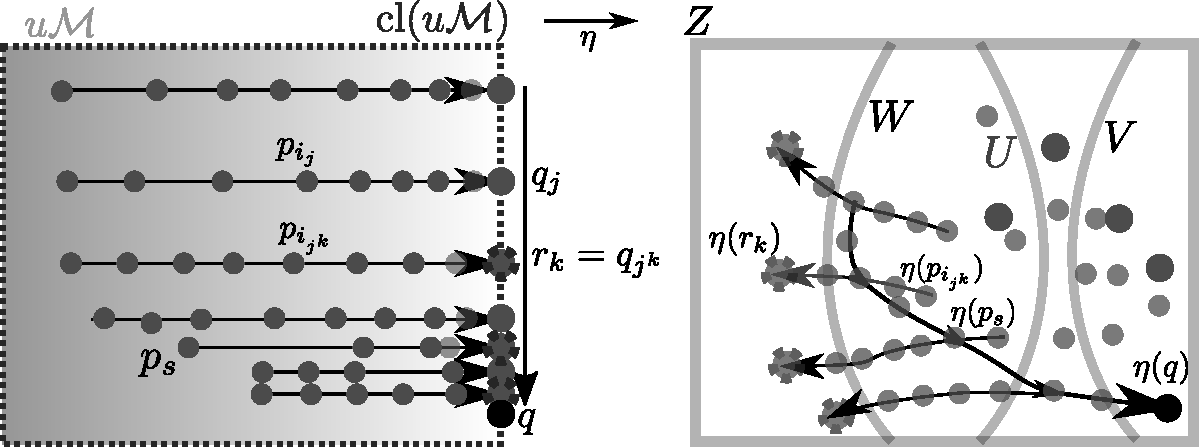
\includegraphics[width={\textwidth}]{drawingbw.pdf}
		{Illustration of the nets described in the following proof.}
	\end{figure}
	
	\begin{prop}
		\label{prop:strange_cont}
		Let $\zeta\colon \overline{u\cM} \to u\cM $ be the function defined by $\zeta(x)=ux$ and let $\xi\colon u\cM \to Z$ be a continuous function, where $Z$ is a regular (e.g.\ compact, Hausdorff) space and $u\cM $ is equipped with the $\tau$-topology. Then $\xi \circ \zeta:\overline{u\cM} \to Z$ is continuous, where $\overline{u\cM}$ is equipped with the topology induced from the Ellis semigroup $EL$.
		
		In particular, the function $\overline{u\cM}\to u\cM/H(u\cM)$, $f\mapsto ufH(u\cM)$ is continuous.
	\end{prop}
	\begin{proof}
		Denote $\xi \circ \zeta$ by $\eta$.
		By Fact~\ref{fct:ulimit}, we know that for any net $(p_i)_i$ in $u\cM $ and $ p \in \overline{u\cM}$ such that $\lim p_i = p$ one has $\tau\mbox{-}\!\lim p_i=up$. So, in such a situation, $\eta(p)=\xi(up)=\lim_i \xi(p_i)=\lim_i \xi(up_i)=\lim_i \eta(p_i)$.
		
		Consider any net $(q_j)_{j\in J}$ in $\overline{u\cM}$ converging to $q$ in $\overline{u\cM}$. The goal is to show that $\lim_j \eta(q_j)=\eta(q)$. Suppose for a contradiction that there is an open neighbourhood $W$ of $\eta(q)$ and a subnet $(r_k)$ of $(q_j)$ such that all points $\eta(r_k)$ belong to $W^c$. Since $Z$ is regular, we can find open subsets $U$ and $V$ such that $W^c \subseteq U$, $\eta(q) \in V$ and $U \cap V=\emptyset$.
		
		For each $j$ we can choose a net $(p_{i^j})_{i^j \in I^j}$ in $u\cM $ such that $\lim_{i^j} p_{i^j}=q_j$.
		
		For each $k$, $r_k = q_{j_{k}}$ for some $j_k \in J$, and $\eta(r_k) \in U$. Hence, since by the first paragraph of the proof $\eta(r_k)=\eta(q_{j_k})= \lim_{i^{j_k}} \eta(p_{i^{j_k}})$, we see that for big enough $i^{j_k} \in I^{j_k}$ one has $\eta(p_{i^{j_k}}) \in U$.
		
		On the other hand, let $S:=J \times \prod_{j \in J} I^j$ be equipped with the product order. For $s \in S$, put $p_s:= p_{i^{j_s}}$, where $j_s$ is the first coordinate of $s$ and $i^{j_s}$ is the $j_s$-coordinate of $s$. Since $\lim_{j \in J} q_j=q$ and $\lim_{i^j \in I^j} p_{i^j}=q_j$, we get $\lim_s p_s=q$. So, by the first paragraph of the proof, $\lim_s \eta(p_s)=\eta(q) $, and hence, for $s\in S$ big enough, $\eta(p_s) \in V$.
		
		By the last two paragraphs, we can find $j \in J$ and $i^j \in I^j$ (big enough) so that $\eta(p_{i^j}) \in U \cap V$, a contradiction, as the last set is empty.
	\end{proof}

	\chapter{Side results}
	\label{app:side}
	This appendix contains various results which have turned up in the context of the thesis, but remain tangential to the main results.
	
	\section[On the existence of a semigroup structure on the type space \texorpdfstring{${S_{\bar c}(\mathfrak{C})}$}{Sc(C)}]{On the existence of a semigroup structure on the type space \texorpdfstring{${S_{\bar c}(\mathfrak{C})}$}{Sc(C)}}
	\sectionmark{Semigroup structure on ${S_{{\bar c}}(\mathfrak{C})}$}
	\label{section: semigroup operation}
	This section was originally the appendix in \cite{KPR15} (joint with Krzysztof Krupiński and Anand Pillay). The original proof of Corollary~\ref{cor:smt_type} in that paper used what we may consider an application of Lemma~\ref{lem:weakly_grouplike} to the case of the $\Aut(\fC)$-ambit $(\Aut(\fC),S_{\bar c}(\fC),\tp(\bar c/\fC))$, where $\fC$ is the monster model and $\bar c$ is its enumeration. In particular, it used the enveloping semigroup $E(\Aut(\fC),S_{\bar c}(\fC))$. In many natural cases, the enveloping semigroup of a dynamical system is naturally isomorphic to that system itself. For example, if we consider $(G,\beta G)$, then $E(G,\beta G)\cong \beta G$.
	
	The question that arises is whether or not $S_{\bar c}(\fC)$ is its own Ellis semigroup, or in other words, whether it admits a left topological semigroup structure (compatible with the action of $\Aut(\fC)$). In this section, we show that the answer is no, unless the underlying theory is stable (in which case, the answer is yes).
	
	The general idea is as follows. We establish the inclusion of $\Aut(\fC)$ in the type space $S_{\bar c}(\fC)$ as a universal object in a certain category. This allows us to describe the existence of a semigroup operation on $S_{\bar c}(\fC)$ in terms of a ``definability of types'' kind of statement, which in turn can be related to stability using a type counting argument.
	
	\begin{prop}\label{proposition: category C}
		Consider $\Aut(\fC)\subseteq S_{\bar c}(\fC)$ given by $\sigma \mapsto \tp(\sigma(\bar c)/\fC)$.
		Consider the category $\catg$ whose objects are maps $\Aut(\fC)\to K$ such that:
		\begin{itemize}
			\item
			$K$ is a compact, zero-dimensional, Hausdorff space,
			\item
			preimages of clopen sets in $K$ are relatively $\fC$-definable in $\Aut(\fC)$, i.e.\ for each clopen $C$ there is a formula $\varphi(x,a)$ with $a$ from $\fC$ such that $\sigma$ is in the preimage of $C$ if and only if $\models \varphi(\sigma(\bar c),a)$,
		\end{itemize}
		where morphisms are continuous maps between target spaces with the obvious commutativity property.
		Then the inclusion of $\Aut(\fC)$ into the space $S_{\bar c}(\fC)$ is the initial object of $\catg$.
	\end{prop}
	\begin{proof}
		Firstly, $\Aut(\fC)$ is dense in $S_{\bar c}(\fC)$, so the uniqueness part of the universal property is immediate. What is left to show is that for every $h\colon \Aut(\fC)\to K$, $h\in \catg$, we can find a continuous map $\bar h\colon S_{\bar c}(\fC)\to K$ extending $h$.
		
		Choose any $p\in S_{\bar c}(\fC)$ and consider it as an ultrafilter
		on relatively $\fC$-definable subsets of $\Aut(\fC)$, and then consider $K_p:=\bigcap \left\{\overline{h[D]}\mid D\in p\right\}\subseteq K$.
		It is the intersection of a centered (i.e.\ with the finite intersection property) family of nonempty, closed subsets of $K$, so it is nonempty. In fact, it is a singleton.
		If not, there are two distinct elements $k_1,k_2 \in K_p$. Take a clopen neighbourhood $U$ of $k_1$ such that $k_2 \notin U$. Since $h \in \catg$, $h^{-1}[U]= \{\sigma \in \Aut(\fC) \mid \;\models \varphi(\sigma(\bar c),a)\}$ for some formula $\varphi(\bar x, a)$. If $\varphi(\bar x, a) \in p$, then $K_p \subseteq \overline{h[h^{-1}[U]]} \subseteq \overline{U}=U$, a contradiction as $k_2 \notin U$. If $\neg \varphi(\bar x, a) \in p$, then $K_p \subseteq \overline{h[\Aut(\fC) \setminus h^{-1}[U]]} \subseteq \overline{K \setminus U}=K \setminus U$, a contradiction as $k_1 \notin K \setminus U$.
		In conclusion, we can define $\bar h(p)$ to be the unique point in $K_p$.
		
		We see that $\bar h$ extends $h$. Moreover, $\bar h$ is continuous, because the preimage of a clopen set $C\subseteq K$ is the basic open set in $S_{\bar c}(\fC)$ corresponding to the relatively definable set $h^{-1}[C]$.
	\end{proof}
	
	In Corollary~\ref{cor: semigroup iff definability of types}, we will establish the aforementioned ``definability of types''-like condition from the existence of a semigroup operation.
	For this we will need the following definition.
	
	
	\begin{dfn}
		\index{piecewise definable type}
		Let $M$ be a model (e.g.\ $M=\fC$). A type $q(x) \in S(M)$ is {\em piecewise definable} if for every type $p(y)\in S(\emptyset)$ and formula $\varphi(x,y)$ the set of $a \in p(M)$ for which $q\vdash \varphi(x,a)$ is relatively $M$-definable in $p(M)$ (that is, there is a formula $\delta(y,c)$ (with $c$ from $M$) such that for any $a\in p(M)$ we have $q\vdash \varphi(x,a)$ if and only if $\delta(a,c)$).\xqed{\lozenge}
	\end{dfn}
	
	
	\begin{rem}\label{remark: piecewise weak definability equals piecewise definability}
		Let $q(x) \in S(\fC)$. The following conditions are equivalent.
		\begin{enumerate}
			\item $q(x)$ is piecewise definable.
			\item For every type $p(y)\in S(\emptyset)$ and formula $\varphi(x,y)$ there is a type $\bar p(yz) \in S(\emptyset)$ extending $p(y)$ such that the set of $ab \models \bar p$ for which $q\vdash \varphi(x,a)$ is relatively $\fC$-definable in $\bar p(\fC)$ (that is, there is a formula $\delta(yz,c)$ (with $c$ from $\fC$) such that for any $ab \models \bar p$ we have $q\vdash \varphi(x,a)$ if and only if $\delta(ab,c)$).
			\item For every $\varphi(x,y)$ and every $a$ from $\fC$ there is some $b$ from $\fC$ such that the set of all $a'b'$ from $\fC$ with $a'b'\equiv ab$ and $q\vdash \varphi(x,a')$ is relatively definable over $\fC$ (among all $a'b'$ from $\fC$ equivalent to $ab$).
		\end{enumerate}\xqed{\lozenge}
	\end{rem}
	
	\begin{proof}
		The equivalence $(2) \Leftrightarrow (3)$ is obvious. It is also clear that $(1) \Rightarrow (2)$, by taking $z$ and $b$ to be empty in (2). It remains to prove $(2) \Rightarrow (1)$.
		
		Take any type $p(y) \in S(\emptyset)$ and formula $\varphi(x,y)$. By (2), there is a type $\bar p(yz) \in S(\emptyset)$ extending $p(y)$ and a formula $\delta(yz,c)$ (with $c$ from $\fC$) such that for any $ab \models \bar p$ we have $q\vdash \varphi(x,a)$ if and only if $\delta(ab,c)$. This implies that for any $a,b,b'$ such that $ab \models \bar p$ and $ab' \models \bar p$ we have $\delta(ab,c) \leftrightarrow \delta(ab',c)$. By compactness, there is a formula $\psi(y,z) \in \bar p(yz)$ such that for any $a,b,b'$ with $ab \models \psi(y,z)$ and $ab' \models \psi(y,z)$ we have $\delta(ab,c) \leftrightarrow \delta(ab',c)$. Put
		$$\delta'(y,c) : = (\exists z) (\psi(y,z) \wedge \delta(yz,c)).$$
		It remains to check that for any $a \models p$, $q\vdash \varphi(x,a)$ if and only if $\delta'(a,c)$.
		
		First, assume $q\vdash \varphi(x,a)$ and $a \models p$. Take $b$ such that $ab \models \bar p$. Then $\psi(a,b) \wedge \delta(ab,c)$, and so $\delta'(a,c)$.
		
		Now, assume that $\delta'(a,c)$ and $a \models p$. Then there is $b$ such that $\psi(a,b)$ and $\delta(ab,c)$. There is also $b'$ with $ab' \models \bar p$, and then $\psi(a,b')$. By the choice of $\psi$, we conclude that $\delta(ab',c)$. Hence, $q\vdash \varphi(x,a)$.
	\end{proof}
	
	
	
	
	\begin{cor}\label{cor: semigroup iff definability of types}
		The natural action $\Aut(\fC)\times S_{\bar c}(\fC)\to S_{\bar c}(\fC)$ extends to a left-continuous semigroup operation on $S_{\bar c}(\fC)$ if and only if each complete type over $\fC$ is piecewise definable.
	\end{cor}
	
	\begin{proof}
		First, using Proposition~\ref{proposition: category C}, we will easily deduce:
		\begin{clm*}
			The action $\Aut(\fC)\times S_{\bar c}(\fC)\to S_{\bar c}(\fC)$ extends to a left-continuous semigroup operation on $S_{\bar c}(\fC)$ if and only if for each $q\in S_{\bar c}(\fC)$ the mapping $h_q \colon \Aut(\fC)\to S_{\bar c}(\fC)$ given by $\sigma \mapsto \sigma(q)$ is in the category $\catg$ (i.e.\ the preimages of clopen sets are relatively $\fC$-definable).
		\end{clm*}
		
		\begin{clmproof}[Proof of claim]
			$(\Rightarrow)$ Let $*$ be a left-continuous semigroup operation on $S_{\bar c}(\fC)$ extending the action of $\Aut(\fC)$. Consider any $q \in S_{\bar c}(\fC)$. Define $\bar h_q \colon S_{\bar c}(\fC) \to S_{\bar c}(\fC)$ by $\bar h_q(p) := p*q$. Then $\bar h_q$ is a continuous extension of $h_q$. By continuity, the preimages of clopen sets by $\bar h_q$ are clopen, and therefore their intersections with $\Aut(\fC)$ (which are exactly the preimages of clopen sets by the original map $h_q$) are relatively $\fC$-definable.
			
			$(\Leftarrow)$ By Proposition~\ref{proposition: category C}, for any $q \in S_{\bar c}(\fC)$ there exists a continuous function $\bar h_q \colon S_{\bar c}(\fC) \to S_{\bar c}(\fC)$ which extends $h_q$. For $p,q \in S_{\bar c}(\fC)$ define $p*q := \bar h_q(p)$. It is clear that $*$ (treated as a two-variable function) is left continuous and extends the action of $\Aut(\fC)$ on $S_{\bar c}(\fC)$. We leave as a standard exercise on limits of nets to check that $*$ is also associative.
		\end{clmproof}
		
		By the claim and Remark~\ref{remark: piecewise weak definability equals piecewise definability}, the whole proof boils down to showing that for any type $q(x) \in S_{\bar c}(\fC)$ we have the following equivalence: the preimage by $h_q$ of any clopen subset of $S_{\bar c}(\fC)$ is relatively definable in $\Aut(\fC)$ if and only if $q(x)$ satisfies item (3) of Remark~\ref{remark: piecewise weak definability equals piecewise definability}.
		
		
		Let us fix an arbitrary $q(x) \in S_{\bar c}(\fC)$, and any formula $\varphi(x,a)$ for some
		$a$ from $\fC$. The preimage by $h_q$ of the clopen set $[\varphi(x,a)]$ equals
		\[
		\{\sigma \in \Aut(\fC)\mid \sigma(q)\vdash \varphi(x,a)\}=\{\sigma \in \Aut(\fC)\mid q\vdash \varphi(x,\sigma^{-1}(a))\}.
		\]
		
		Now, for $(\Leftarrow)$, suppose there is some $b$ from $\fC$ and a formula $\delta(yz,c)$ (with $c$ from $\fC$) such that for any $a'b'\equiv ab$ we have $q\vdash \varphi(x,a')$ if and only if $\models \delta(a'b',c)$. Then (taking $a'b'=\sigma^{-1}(ab)$) we have that
		\[
		q\vdash \varphi(x,\sigma^{-1}(a))\iff \models \delta(\sigma^{-1}(ab),c)\iff \models \delta(ab,\sigma(c)),
		\]
		and the last statement is clearly relatively $\fC$-definable about $\sigma$.
		
		For $(\Rightarrow)$, suppose $\{\sigma\in \Aut(\fC)\mid q\vdash \varphi(x,\sigma^{-1}(a))\}$ is defined by some formula $\delta$, i.e.\ for some $d,c$ from $\fC$, for any $\sigma \in \Aut(\fC)$ we have
		\[
		q\vdash \varphi(x,\sigma^{-1}(a))\iff \models\delta(d,\sigma(c)) \iff \models \delta(\sigma^{-1}(d),c).
		\]
		We can assume without loss of generality that $d=ab$ for some $b$ from $\fC$ (adding dummy variables to $\delta$ if necessary). But then, for $a'b'\equiv ab$ there is some automorphism $\sigma$ such that $\sigma(a'b')=ab$, so we have
		\[
		q\vdash \varphi(x,a')\iff \models \delta(a'b',c).\qedhere
		\]
	\end{proof}
	
	This easily implies that stability is sufficient for the existence of a semigroup structure.
	
	\begin{cor}\label{corollary: stability implies semigroup}
		If $T$ is stable, then $S_{\bar c}(\fC)$ has a left-continuous semigroup operation extending the action of $\Aut(\fC)$ on $S_{\bar c}(\fC)$
	\end{cor}
	\begin{proof}
		If $T$ is stable, then every type over $\fC$ is definable, so in particular it is piecewise definable, which by Corollary~\ref{cor: semigroup iff definability of types} implies that the semigroup structure exists.
	\end{proof}
	
	For the other direction, we will use Corollary~\ref{cor: semigroup iff definability of types} and an easy counting argument. But before that we need to establish a transfer property for piecewise definability.
	
	\begin{prop}\label{proposition: transfer of piecewise definability}
		Suppose that each complete type over $\fC$ is piecewise definable. Then each complete type over any model $M$ of cardinality less then $\kappa$ (where $\kappa$ is the degree of saturation of $\fC$) is piecewise definable.
	\end{prop}
	
	\begin{proof}
		Take any $q(x) \in S(M)$.
		Consider any type $p(y) \in S(\emptyset)$ and formula $\varphi(x,y)$.
		Take a coheir extension $\bar q \in S(\fC)$ of $q$. Then $q$ is invariant over $M$. By assumption, $\bar q$ is piecewise definable. So there is a formula $\delta(y,c)$ (with $c$ from $\fC$) such that for any $a \in p(\fC)$, $\bar q\vdash \varphi(x,a)$ if and only if $\delta(a,c)$. Denote by $A$ the set of all $a \in p(\fC)$ satisfying these equivalent conditions; so $A$ is a relatively definable subset of $p(\fC)$. By the invariance of $\bar q$ over $M$, we see that $A$ is invariant over $M$, and so, by $\kappa$-saturation and strong $\kappa$-homogeneity of $\fC$, the subset $A$ of $p(\fC)$ is relatively definable over $M$. In other words, there is a formula $\delta'(y,m)$ (with $m$ from $M$) such that for any $a \in p(\fC)$, $\bar q\vdash \varphi(x,a)$ if and only if $\delta'(a,m)$. Hence, for any $a \in p(M)$, $q\vdash \varphi(x,a)$ if and only if $\delta'(a,m)$.
	\end{proof}
	
	\begin{cor}\label{cor: semigroup = stability}
		$S_{\bar c}(\fC)$ has a left-continuous semigroup operation extending the action of $\Aut(\fC)$ on $S_{\bar c}(\fC)$ if and only if $T$ is stable.
	\end{cor}
	\begin{proof}
		The ``if'' part is the content of Corollary~\ref{corollary: stability implies semigroup}.
		
		$(\Rightarrow)$ Assume $S_{\bar c}(\fC)$ has a left-continuous semigroup operation extending the action of $\Aut(\fC)$ on $S_{\bar c}(\fC)$. Then, by Corollary~\ref{cor: semigroup iff definability of types}, all complete types over $\fC$ are piecewise definable. We will show that this implies that $T$ is $\beth_2(|T|)$-stable (where $\beth_2(|T|): = 2^{2^{|T|}}$). Consider any $M \models T$ of cardinality at most $\beth_2(|T|)$. We need to show that $|S_1(M)| \leq \beth_2(|T|)$. For this it is enough to prove that for any $\varphi(x,y)$ (where $x$ is a single variable) $|S_\varphi(M)| \leq \beth_2(|T|)$. Without loss of generality $M \prec \fC$.
		%
		By Proposition~\ref{proposition: transfer of piecewise definability}, each complete type over $M$ is piecewise definable. This implies that each type $q \in S_\varphi(M)$ is determined by a function $S_y(\emptyset) \to \lang(M)$ which takes $p(y)$ to $\delta(y,c)$ witnessing piecewise definability of $q$ (or, more precisely, of an arbitrarily chosen extension of $q$ to a type in $S_1(M)$) for the formula $\varphi(x,y)$. So $|S_\varphi(M)| \leq |\lang(M)|^{|S_y(\emptyset)|} \leq (\beth_2(|T|))^{2^{|T|}}=\beth_2(|T|)$.
	\end{proof}
	
	It is well known that if $T$ is stable, then it is $2^{|T|}$-stable. The reason why we worked with $\beth_2(|T|)$ in the above proof is that this is the ``degree'' of stability which we can deduce directly from piecewise definability. Then, knowing that $T$ is stable, we have the usual definability of types which implies $2^{|T|}$-stability.
	
	
	
	
	\section{Closed group-like implies properly group-like}
	Here, we show that closed group-like equivalence relations form a subclass of properly group-like equivalence relations (in particular, e.g.\ in Lemma~\ref{lem:main_abstract_grouplike}(2), in ``closed or properly group-like'', the ``closed'' part is redundant, and likewise in Lemma~\ref{lem:weakly_grouplike}(2).
	
	\begin{prop}
		\label{prop:closed_glike_is_properly_glike}
		Suppose $(G,X,x_0)$ is an ambit and $E$ is a closed group-like equivalence relation on $X$. Then $E$ is properly group-like.
	\end{prop}
	\begin{proof}
		The proof works via non-standard analysis.
		
		Consider the structure $M=(G,X,\cdot)$, where $G$ has its group structure, while $X$ has predicates for all open subsets of all its powers, and $\cdot\colon G\times X\to X$ is the group action.
		
		Now, given any $N=(G',X',\cdot )\equiv M$, we have a standard part function ${\st}\colon X'\to X$: $\st(x')=x$ when for every open $U\ni x$ we have $x'\in U^N$. By the Hausdorff condition, there is at most one such $x$, and by compactness, it always exists. Moreover, note that if $x'\in U^N$, then $\st(x')\in U$. Similarly, a finite tuple of elements of $X$ also has a standard part (which is the tuple of standard parts of its coordinates).
		
		Now let $M^*=(G^*,X^*,\cdot)\succeq M$ be a highly saturated elementary extension (to be precise, it is enough for it to be saturated in any cardinality greater than the local character of $X$, e.g.\ if $X$ is first-countable, we can take any ultrapower of $M$ with respect to a non-principal ultrafilter). For $\tilde g\in G^*$ let $[\tilde g]_\equiv=\st(\tilde g\cdot x_0)$. We will show that $\tilde G:=G^*$ witnesses proper group-likeness of $E$.
		
		(Note that the action of $G^*$ on $X^*$ generally does \emph{not} give us a well-defined action of $G^*$ on $X$, unless the action of $G$ on $X$ is equicontinuous, as we can have $\st(x_1^*)=\st(x_2^*)$ but $\st(\tilde g\cdot x_1^*)\neq \st(\tilde g\cdot x_2^*)$.)
		
		First, we need to show that $\tilde g\mapsto [\st(\tilde g\cdot x_0)]_E$ is a group homomorphism. Let $\mu\subseteq X^3$ be the set of triples $(x_1,x_2,x_3)$ such that $[x_1]_E\cdot [x_2]_E=[x_3]_E$. Then by group-likeness, for all $g_1,g_2\in G$ we have that $(g_1x_0,g_2x_0,g_1g_2x_0)\in \mu$, and therefore, for any open $U\supseteq \mu$ we have $(g_1x_0,g_2x_0,g_1g_2x_0)\in U$. By elementarity, for all $\tilde g_1,\tilde g_2\in G^*$ we have that $(\tilde g_1x_0,\tilde g_2x_0,\tilde g_1\tilde g_2 x_0)\in U^*$, where $U^*=U^{M^*}$. By the preceding remarks, we have also that $(\st(\tilde g_1x_0),\st(\tilde g_2x_0),\st(\tilde g_1\tilde g_2x_0))\in U$.
		
		Now, since $X/E$ is a Hausdorff topological group, the graph of its multiplication is closed, and it follows that $\mu$ is closed, and as such (because $X$ is compact Hausdorff), it is equal to the intersection of all the open sets contained it, so (because $U$ in the preceding paragraph was arbitrary) in fact, we have for any $\tilde g_1,\tilde g_2$ that $(\st(\tilde g_1x_0),\st(\tilde g_2x_0),\st(\tilde g_1\tilde g_2x_0))\in \mu$, i.e.\ $[\st(\tilde g_1x_0)]_E\cdot [\st(\tilde g_2x_0)]_E=[\st(\tilde g_1\tilde g_2 x_0)]_E$.
		
		To show that we have pseudocompleteness, note that if we have for some nets $g_ix_0\to x_1$ and $p_i\to x_2$ and $g_i\cdot p_i\to x_3$, for any open neighbourhoods $U_1,U_2,U_3$ of $x_1,x_2,x_3$ (respectively), there are $g',g''\in G$ such that $g'x_0\in U_1$, $g''x_0\in U_2$ and $g'g''x_0\in U_3$. Indeed, if we take any $i$ such that $g_ix_0\in U_1$, $p_i\in U_2$ and $g_ip_i\in U_3$, then we can take $g'=g_i$ and $g''$ such that $g''x_0\in U_2\cap g_i^{-1}[U_3]\ni p_i$ (which exist because $(X,x_0)$ is a $G$-ambit, and $U_2\cap g_i^{-1}[U_3]$ is a nonempty open set).
		
		It follows by compactness that we have $\tilde g_1,\tilde g_2\in G^*$ such that $\st(\tilde g_1\cdot x_0)=x_1$, $\st(\tilde g_2\cdot x_0)=x_2$ and $\st(\tilde g_1\tilde g_2\cdot x_0)=x_3$, which gives us pseudocompleteness.
		
		For the final part, note that $[\tilde g_1]_\equiv=[\tilde g_2]_\equiv$ means just that for every open $U\subseteq X$ we have that $\tilde g_1\cdot x_0\in U^*\leftrightarrow \tilde g_2\cdot x_0\in U^*$, which is a type-definable condition. Thus $F_0'=\{ \tilde g_1^{-1}\tilde g_2x_0\mid [\tilde g_1]_\equiv=[\tilde g_2]_\equiv \}$ is a type-definable set, so by compactness, $F_0=\{\st(x^*)\mid x^*\in F_0' \}$ is closed.
	\end{proof}
	
	Note that if $E$ is closed group-like, then $E$ itself is a symmetric closed set containing the diagonal and $E\circ E=E$, so $\mathcal E=\{E\}$ could conceivably witness \emph{uniformly} proper group-likeness of $E$ (according to Definition~\ref{dfn:unif_prop_glike}). Furthermore, closed group-like equivalence relations share many properties of uniformly properly group-like equivalence relations. This suggests the following question.
	
	\begin{qu}
		\label{qu:clsd_gplike_upglike}
		Are closed group-like equivalence relations uniformly properly group-like?
	\end{qu}

	The problem is that it is not clear how to choose $\tilde G$: we would need to have that for every $\tilde g\in \tilde G$ such that $[\tilde g]_{\equiv}\Er x_0$, for every other $\tilde g'\in \tilde G$, $[\tilde g']_{\equiv}\Er [\tilde g\tilde g']_{\equiv}$
	
	Note that for $\tilde G=G^*$ as in the proof of Proposition~\ref{prop:closed_glike_is_properly_glike}, there seems to be no obvious reason for this to be true.
	
	
